In this section, we present the adversary model and the design goal. In this paper, we consider fault localization for end-to-end communication in multi-hop networks, where packets are delivered through a set of intermediate routers \emph{R}$_\emph{i}$ (1$\leq \emph{i} \leq$\emph{n}) between a source {\tt S} and a destination {\tt D},  where \emph{n} is the path length (not including {\tt S} and {\tt D}), and {\tt S}, {\tt D} and \emph{R}$_\emph{i}$ are network entities in a network.  
%We denote the source by {\tt S}, the routers in a path by \emph{R}$_\emph{i}$ (1$\leq \emph{i} \leq$\emph{n}) and the destination by {\tt D}, where \emph{n} is the path length (not including {\tt S} and {\tt D}). 
%. 
Under an unreliable communication channel, a network entity may drop, modify, and hijack  forwarding packets, which is usually incurred by attacks or network failure (e.g., misconfiguration and link failure). Both compromised and misconfigured entities are treated as misbehaved entities because they incur packet forwarding anomalies. 
%the compromised router controlled by an adversary can launch source spoofing and packet hijacking attacks, and the misconfigured router has security threat for data-plane path compliance..
%\vspace{-0.1in}
\begin{figure}%[H]
\begin{center}
  % Requires \usepackage{graphicx}
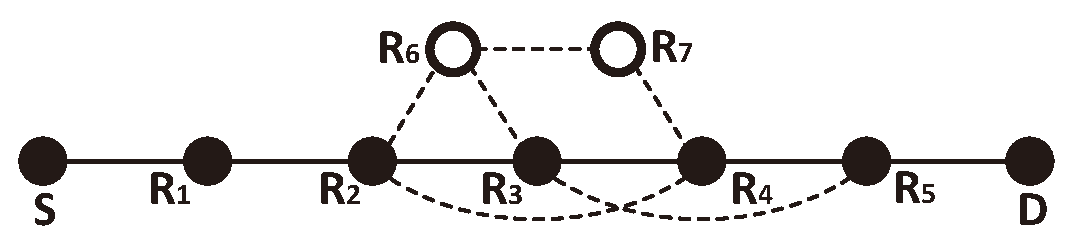
\includegraphics[width=7cm]{visio/attackmodel3.eps}
\caption{Adversary model where \emph{R}$_\emph{2}$ is the misbehaved entity and the purposed forwarding path is $\Psi$ \emph{=} $\langle$\emph{R}$_\emph{1}$\emph{, R}$_\emph{2}$\emph{, R}$_\emph{3}$\emph{, R}$_\emph{4}$\emph{, R}$_\emph{5}\rangle$ between {\tt S} and {\tt D}.}\label{attackmodel}
\end{center}
\vspace{-3mm}
\end{figure}
\vspace{-0.1in}
\subsection{Adversary Model}
In this paper, we focus on fault localization by performing packet delivery verification, which ensures source authenticity and correct packet forwarding. Intuitively, Fig. \ref{attackmodel} shows  examples of attacks. We assume \emph{R}$_\emph{2}$ is the misbehaved entity. and $\Psi$ \emph{=} $\langle$\emph{R}$_\emph{1}$\emph{, R}$_\emph{2}$\emph{, R}$_\emph{3}$\emph{, R}$_\emph{4}$\emph{, R}$_\emph{5}\rangle$, where $\Psi$ is the desired forwarding path. In this case, \emph{R}$_\emph{2}$ can modify the source address of IP packets originating from {\tt S} for launching \textbf{source spoofing} attack. Besides, \emph{R}$_\emph{2}$ can make the packets delivered along a path that differs from $\Psi$, e.g., $\langle$\emph{R}$_\emph{2}$\emph{, R}$_\emph{6}$\emph{, R}$_\emph{3}$$\rangle$, $\langle$\emph{R}$_\emph{2}$\emph{, R}$_\emph{6}$\emph{, R}$_\emph{7}$\emph{, R}$_\emph{4}$$\rangle$ and $\langle$\emph{R}$_\emph{2}$\emph{, R}$_\emph{4}\rangle$ for the purpose of \textbf{path inconsistency}\footnote{Traffic hijacking is one of the instantiations of forwarding path inconsistency attack.} attack. Moreover, if more than one misbehaved entities occur on $\Psi$, the packets can be transmitted along the unordered entities, e.g., $\langle$\emph{R}$_\emph{2}$\emph{, R}$_\emph{4}$\emph{, R}$_\emph{3}$\emph{, R}$_\emph{5}\rangle$.

As packets may be forwarded on unreliable communication channels, in particular, adversaries may interfere with fault localization, it is difficult to identify misbehaved entities. %localizing the misbehaved entity can be interfered if any fault occurs.}
%During the packet forwarding verification, localizing the misbehaved entity is a higher requirement if any error occurs. However, 
%In this case, 
The misbehaved entity can launch various \textbf{sophisticated attacks} to evade to be localized. In details, the attacks can be classified into two categories.
Firstly, the misbehaved entity can destroy or disturb fault localization by unexpectedly discarding, modifying and redirecting some messages used to localize the fault. For example, when {\tt S} tries to establish symmetric keys with intermediate entities on $\Psi$, \emph{R}$_\emph{2}$ can drop \emph{request} packets (from {\tt S} to \emph{R}$_\emph{i}$) or \emph{ack} packets (from \emph{R}$_\emph{i}$ to {\tt S}) to destroy this procedure of key distribution; or when \emph{R}$_\emph{3}$ reports \emph{ack} packet to {\tt S}, \emph{R}$_\emph{2}$ can modify this packet data to disturb the fault localization.
Secondly, the misbehaved entity can frame benign entities of their unrealistic misbehavior by launching frame attack. For example, when receiving a packet, \emph{R}$_\emph{2}$ greatly reduces the TTL value to 2, causing the illusion that \emph{R}$_\emph{4}$ is regarded as the fault due to its dropping the packet.
\vspace{-0.1in}
\subsection{Design Goal}
\label{desiredproperties}
To defend against the above adversary model, the following desired properties should be satisfied in fault localization. 

\noindent\textbf{Source and path verification.} Each entity on $\Psi$ can perform source and path verification. Once source spoofing or path inconsistency occurs, the entity can identify and filter the unreliable packets. 

%Note that, end-to-end communication sessions can be divided into consecutive \textbf{\emph{epochs}} that vary in different sessions and their phases. We perform the verification during each epoch. In one session, after {\tt S} sends an amount of packets to {\tt D} or a period of time interval expires, the \emph{epoch} value would be updated. 
\noindent\textbf{High accuracy of fault localization.} The source can effectively localize the fault with a high localization accuracy if any error occurs during symmetric key establishment or date forwarding verification. 

\noindent\textbf{Robustness and lightweight.} The fault localization can be robust and anti-attack, which no longer relies on reliable communication channels. Each entity is expectedly lightweight that does not store the symmetric keys shared with other network entities.
%\subsection{Problem Formulation}
%\label{problemformulation}
%This paper focuses on the data-plane fault localization for source authenticity and path compliance. 
%\textcolor{red}{In order to achieve fault localization, we formulate the several problems as the following definition shows.}\\
%\noindent{\textbf{Definition 1.}} We divide the end-to-end communication session into consecutive \textbf{\emph{epoch}}s, which varies with different sessions and their phases. For one session, after a period of time interval or {\tt S} sends an amount of packets to {\tt D}, the \emph{epoch} value would be switched.\\
%\noindent{\textbf{Definition 2.}} The \textbf{\emph{timer}} $\mathcal{T}_\emph{S}$ and $\mathcal{T}_\emph{i}$ are running on {\tt S} and \emph{R}$_\emph{i}$ on $\Psi$, respectively. They starts when the request package arrives and expires after a certain timeout, called \emph{\textbf{timer threshold}} that can be evaluated by a \emph{round-trip time} (RTT).\\ %of the corresponding entity on \emph{Path}$^\emph{*}$.\\
%\noindent{\textbf{Definition 3.}} In this paper, we denote \textbf{\emph{fault localization}} as to localize the misbehaved entity as well as its one neighbor, because accurately localizing the misbehaved entity is impossible to achieve according to the research \cite{barak2008protocols}. Of course, for the higher requirements, centralization-based mechanisms (e.g., VeriDP \cite{zhang2016mind}) in SDN, can be employed, which is not suitable for end-to-end communication.\\
%\noindent{\textbf{Definition 4.}} We define \emph{\textbf{positive ratio}} denoted by $\mathcal{P}_\emph{i}$ and $\mathcal{P}_\emph{D}$ for \emph{R}$_\emph{i}$ and {\tt D}, which illustrates the probability that the corresponding entity is misbehaved. When $\mathcal{P}_\emph{i}$ is larger than \emph{\textbf{positive ratio threshold}} (denoted by $\zeta$), and $\mathcal{P}_\emph{1}$, $\cdots$, $\mathcal{P}_{\emph{i-}1}$ are all less than $\zeta$, we can identify \emph{R}$_\tau$ or \emph{R}$_{\emph{i-}1}$ as the misbehaved entity (detailed in Section \ref{faultlocalization}).
%\vspace{-0.1in}

%In this paper, we focus on \textbf{\emph{fault localization}} as to localize misbehaved entities as well as its  neighbor, 
In this paper, we focus on the data-plane fault localization by verifying source authenticity and path consistency. We treat the detected entity and its neighbor as misbehaved entities because it is impossible to achieve the accuracy to a concrete entity of fault localization as the research \cite{barak2008protocols} describes. 
%Of course, for the higher requirements, centralization-based mechanisms (e.g., VeriDP \cite{zhang2016mind}) in SDN, can be employed, which is not suitable for end-to-end communication.\\
%\subsection{Scope and Assumptions}
%In this paper, we focus on the data-plane fault localization by verifying source authenticity and path consistency.  %while the packet is intended to be delivered through $\Psi$, 
We assume end hosts ({\tt S} and {\tt D}) are trusted because it is meaningless for a malicious source to detect faked packet source and wrong forwarding path. %As we perform data-plane detection, we assume 
Also, {\tt S} should know the packet forwarding path $\Psi$, which can be learned by the existing control-data plane routing protocols \cite{hu2004spv} \cite{murphy1996digital}, or it can be achieved by source routing \cite{sourcerouting}. %Due to the majority of symmetric forwarding path in today's Internet \cite{john2010estimating}, we assume \emph{Path}$^\emph{*}$ is symmetric.
%As for the secret key distribution, we assume the public/private key of 
Meanwhile, each entity on $\Psi$ has long-lived public and private keys, and the public keys can be retrieved and verified by others, which is similar to existing secure routing protocols~\cite{kim2014lightweight} \cite{basescu2016high} \cite{zhang2012shortmac} . 
%In this paper, we employ Dynamically Recreatable Key (DRKey) protocol \cite{kim2014lightweight} to establishes symmetric keys shared between routers and endhosts, in which routers don't need to store the keys that prevents state exhaustion DoS attacks.
%Due to the possible existence of malicious router(s), we assume any attacks can be launched to prevent the data-plane source and path monitoring. For example, the misbehaved router can disturb the symmetric key creation and distribution, and obstruct transmission of acknowledgements from kind nodes. 